\documentclass[journal]{IEEEtran}

\usepackage{amsmath,amssymb,amsfonts}
\usepackage{graphicx}
\usepackage{booktabs}
\usepackage{multirow}
\usepackage{cite}
\usepackage{url}
\usepackage{hyperref}
\usepackage{xcolor}

\hypersetup{
  colorlinks=true,
  linkcolor=blue!50!black,
  citecolor=green!40!black,
  urlcolor=blue!40!black,
}

\newcommand{\argmin}{\operatorname*{arg\,min}}

\title{DSCSP for Diffusion Steganography: \nA Reproducibility-Centered TIFS Manuscript from Current Artifacts}

\author{Anonymous Authors}

\begin{document}
\maketitle

\begin{abstract}
This manuscript reports the current validated state of DSCSP (Diffusion-Stego with Conditional Sampling Paths) using repository-native artifacts rather than legacy draft claims. The primary narrative is the TIFS autopilot v4 line (cycles 1--11), where the best balanced checkpoint (cycle 11, robust\_balance) achieves clean BER $0.0243$, JPEG Q75 BER $0.1370$, and adaptive steganalysis AUC $0.6915$ under the project gate of $\leq 0.70$. However, crop robustness remains unresolved: crop Q80 BER is $0.4955$, near random-guess behavior. Cross-dataset checks are valid but show the same weakness under crop, with CIFAR10 crop BER $0.5020$ and STL10 crop BER $0.5007$. To avoid model-family conflation, we treat v5 outputs as supporting analysis only: short-run ablations and a statistical security report indicate low global distribution shift by KL ($0.417$) but statistically significant spectral discrepancy ($p\approx 1.07\times10^{-122}$) and concentrated perturbation singular spectrum (Gini $0.820$). The resulting evidence supports one positive claim and two open blockers: detectability can be reduced to the target regime in at least one cycle, but crop robustness and quality under that detectability regime are not yet publication-ready. We provide a transparent, failure-aware evaluation template suitable for iterative TIFS hardening.
\end{abstract}

\begin{IEEEkeywords}
Steganography, diffusion models, information forensics, robustness, steganalysis, reproducibility.
\end{IEEEkeywords}

\section{Introduction}
Generative steganography has shifted hidden communication from cover modification to cover synthesis. Diffusion models \cite{ho2020denoising,song2020denoising} are a natural backbone for this direction because they generate high-fidelity images and expose controllable sampling trajectories. The key challenge is not only message recovery but also robustness and detectability under realistic channels and adaptive wardens.

Earlier DSCSP drafts emphasized strong clean/JPEG reconstruction but also documented severe detectability and robustness gaps. In this work, we intentionally rebuild the manuscript from local source-of-truth artifacts: training/evaluation code, autopilot logs, and JSON results. The goal is to avoid stale claims and provide a technically honest TIFS-style report of what is currently validated.

The primary evidence comes from the TIFS autopilot v4 line, where cycle 11 (variant: robust\_balance) reaches adaptive AUC $0.6915$ (passing the project target $\leq 0.70$) while preserving moderate BER performance (clean BER $0.0243$, JPEG Q75 BER $0.1370$). The dominant blocker remains crop robustness, with crop Q80 BER $0.4955$ (target $\leq 0.35$), consistently near chance.

\subsection{Contributions}
\begin{itemize}
\item We provide an artifact-grounded manuscript in which all quantitative claims are directly tied to current code outputs, with explicit separation between the v4 autopilot line (primary) and v5 analyses (supporting).
\item We document an empirical trade-off frontier observed across cycles: BER/JPEG gains can coexist with poor detectability (e.g., cycle 10), while detectability improvements (cycle 11) currently coincide with weaker image quality and unresolved crop BER.
\item We integrate cross-dataset evidence, ablation results, and statistical security diagnostics into one coherent TIFS-oriented reporting stack.
\item We present a transparent limitations section centered on unresolved crop robustness and residual statistical signatures, avoiding unsupported state-of-the-art claims.
\end{itemize}

\section{Related Work}
Classical steganography prioritizes imperceptibility under hand-crafted distortion models \cite{cox2007digital,pevny2010using,holub2012designing,holub2014universal}. Deep learning methods such as HiDDeN and SteganoGAN \cite{zhu2018hidden,zhang2019steganogan} jointly optimize embedding and extraction but still face detectability under strong steganalyzers.

Diffusion-based schemes include training-free projection approaches (Diffusion-Stego) \cite{wei2023diffusionstego} and model-adaptive variants \cite{peng2023stegodiffusion,zhang2024ldstega,zhao2024dero}. In DSCSP, the diffusion model remains frozen and a learned controller applies perturbations at the image level. This design lowers compute requirements but places more burden on controller/extractor learning and attack-aware training.

For detectability, SRM-domain and deep residual steganalysis remain strong baselines \cite{fridrich2012rich,boroumand2019deep}. Adversarial hardening, spectral constraints, and differentiable attack simulation are common directions \cite{goodfellow2014generative,miyato2018spectral,bengio2013estimating,shin2017jpeg}, but robustness under geometric distortions (especially crop-resize) remains difficult in many spatially structured encoders.

\section{Threat Model and Problem Setup}
We consider a sender-receiver pair and a warden.

\textbf{Sender/receiver objective:} embed payload $m\in\{0,1\}^{M}$ into a generated image and recover it after channel distortions.

\textbf{Warden objective:} distinguish clean and stego images. We evaluate adaptive deep steganalysis AUC and treat lower AUC as better concealment.

\textbf{Channel model:} JPEG compression, crop-resize, additive noise, blur, and brightness/contrast transforms. Evaluation emphasizes clean BER, JPEG Q75 BER, crop Q80 BER, and adaptive AUC.

Given a clean image $x_c$ from a frozen diffusion model and a payload encoding $p$, the controller outputs perturbation $\delta=C_\phi(x_c,p)$ and forms stego image
\begin{equation}
  x_s = \mathrm{clip}(x_c + \delta, -1, 1).
\end{equation}
The extractor predicts payload logits $\hat{p}=E_\psi(x_s)$ (or decoded message under redundant coding).

\section{Methodology (Code-Verified)}
\subsection{Primary Architecture Line (v4 Autopilot)}
The primary line uses:
\begin{itemize}
\item Frozen DDPM wrapper with DDIM sampling (20 steps).
\item ContentAdaptiveController (U-Net style encoder-decoder, payload-conditioned and image-conditioned).
\item ResNet-18-based extractor in spatial-map mode.
\item SRM-preprocessed spectral-normalized discriminator when adversarial training is enabled.
\item Differentiable AttackLayer including JPEG, crop-resize, blur, noise, and brightness/contrast.
\end{itemize}

\begin{figure}[t]
\centering
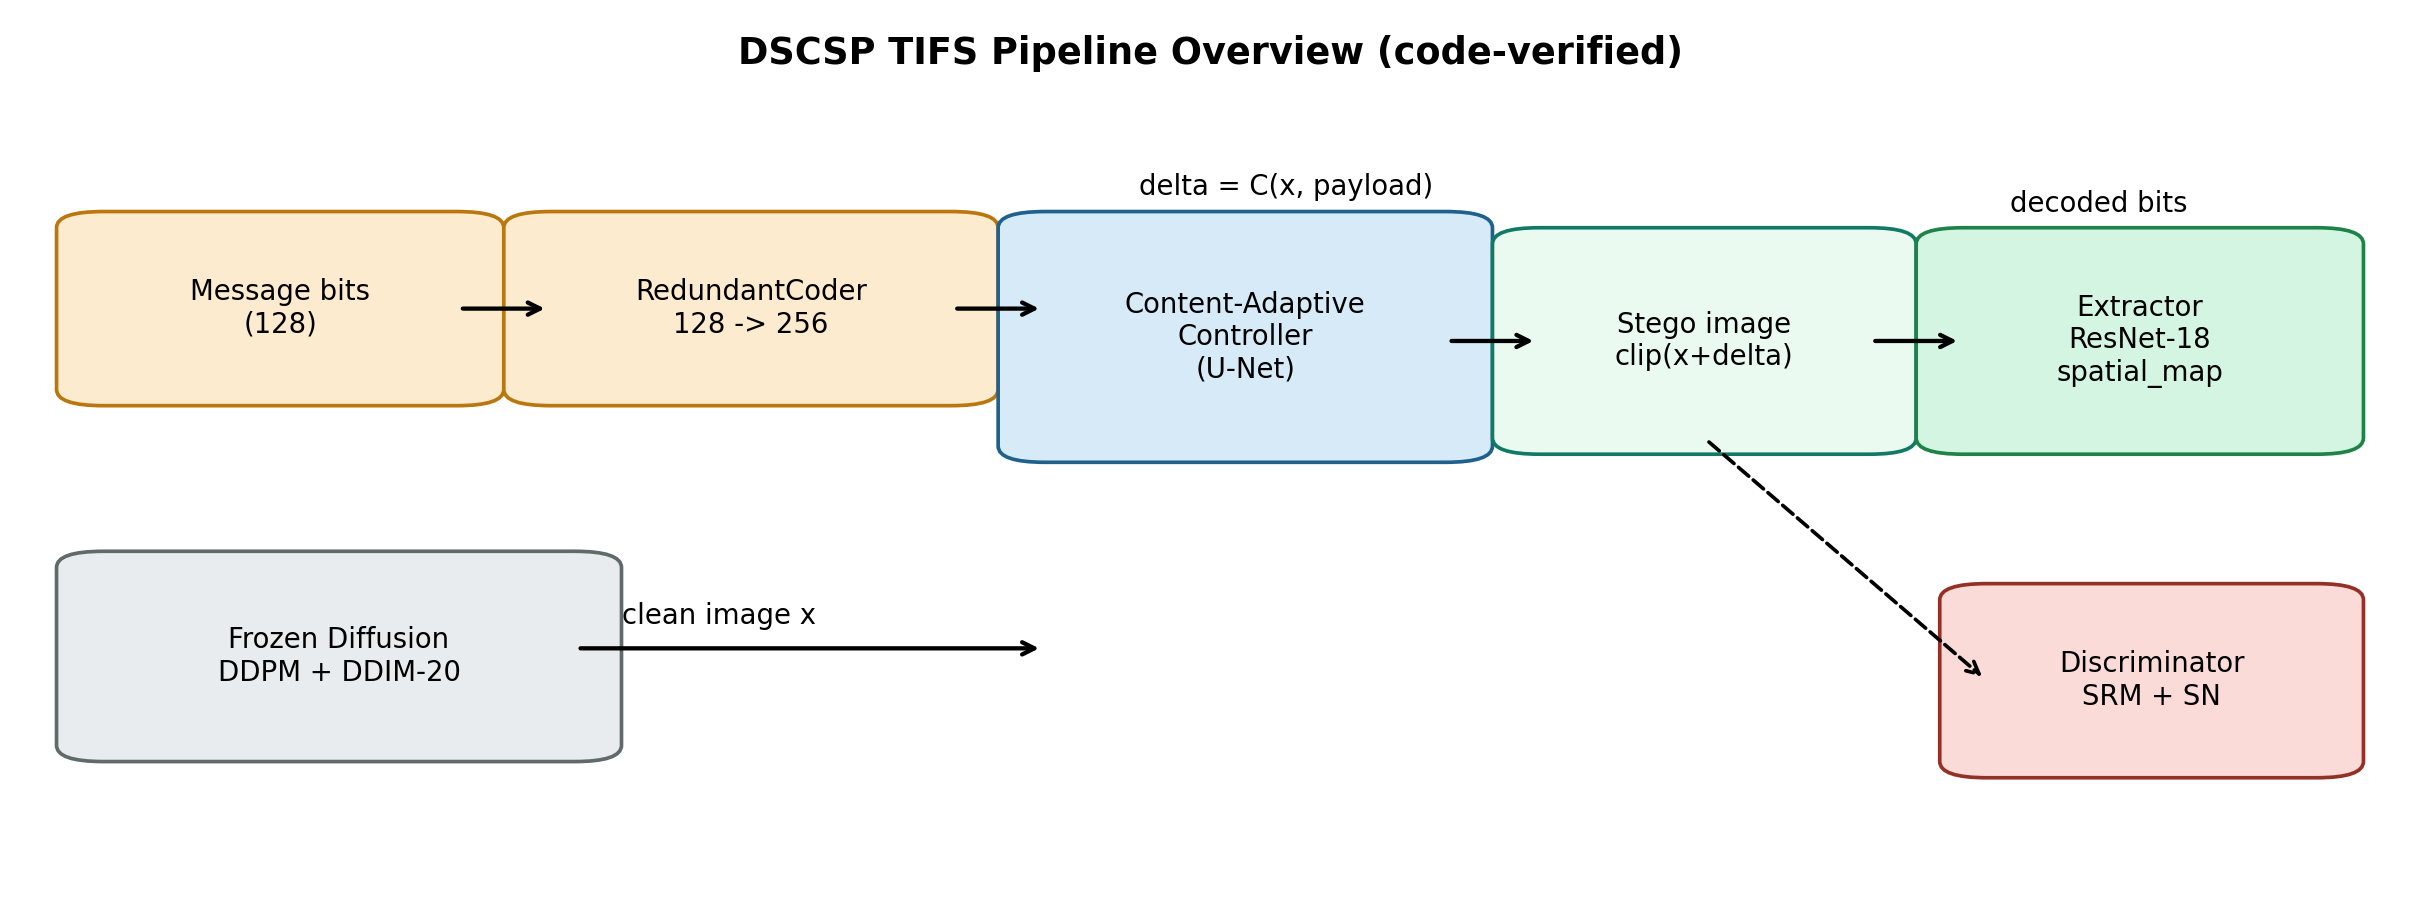
\includegraphics[width=\columnwidth]{figures/system_overview.png}
\caption{System overview generated from current code structure and run configuration.}
\label{fig:system_overview}
\end{figure}

\begin{figure*}[t]
\centering
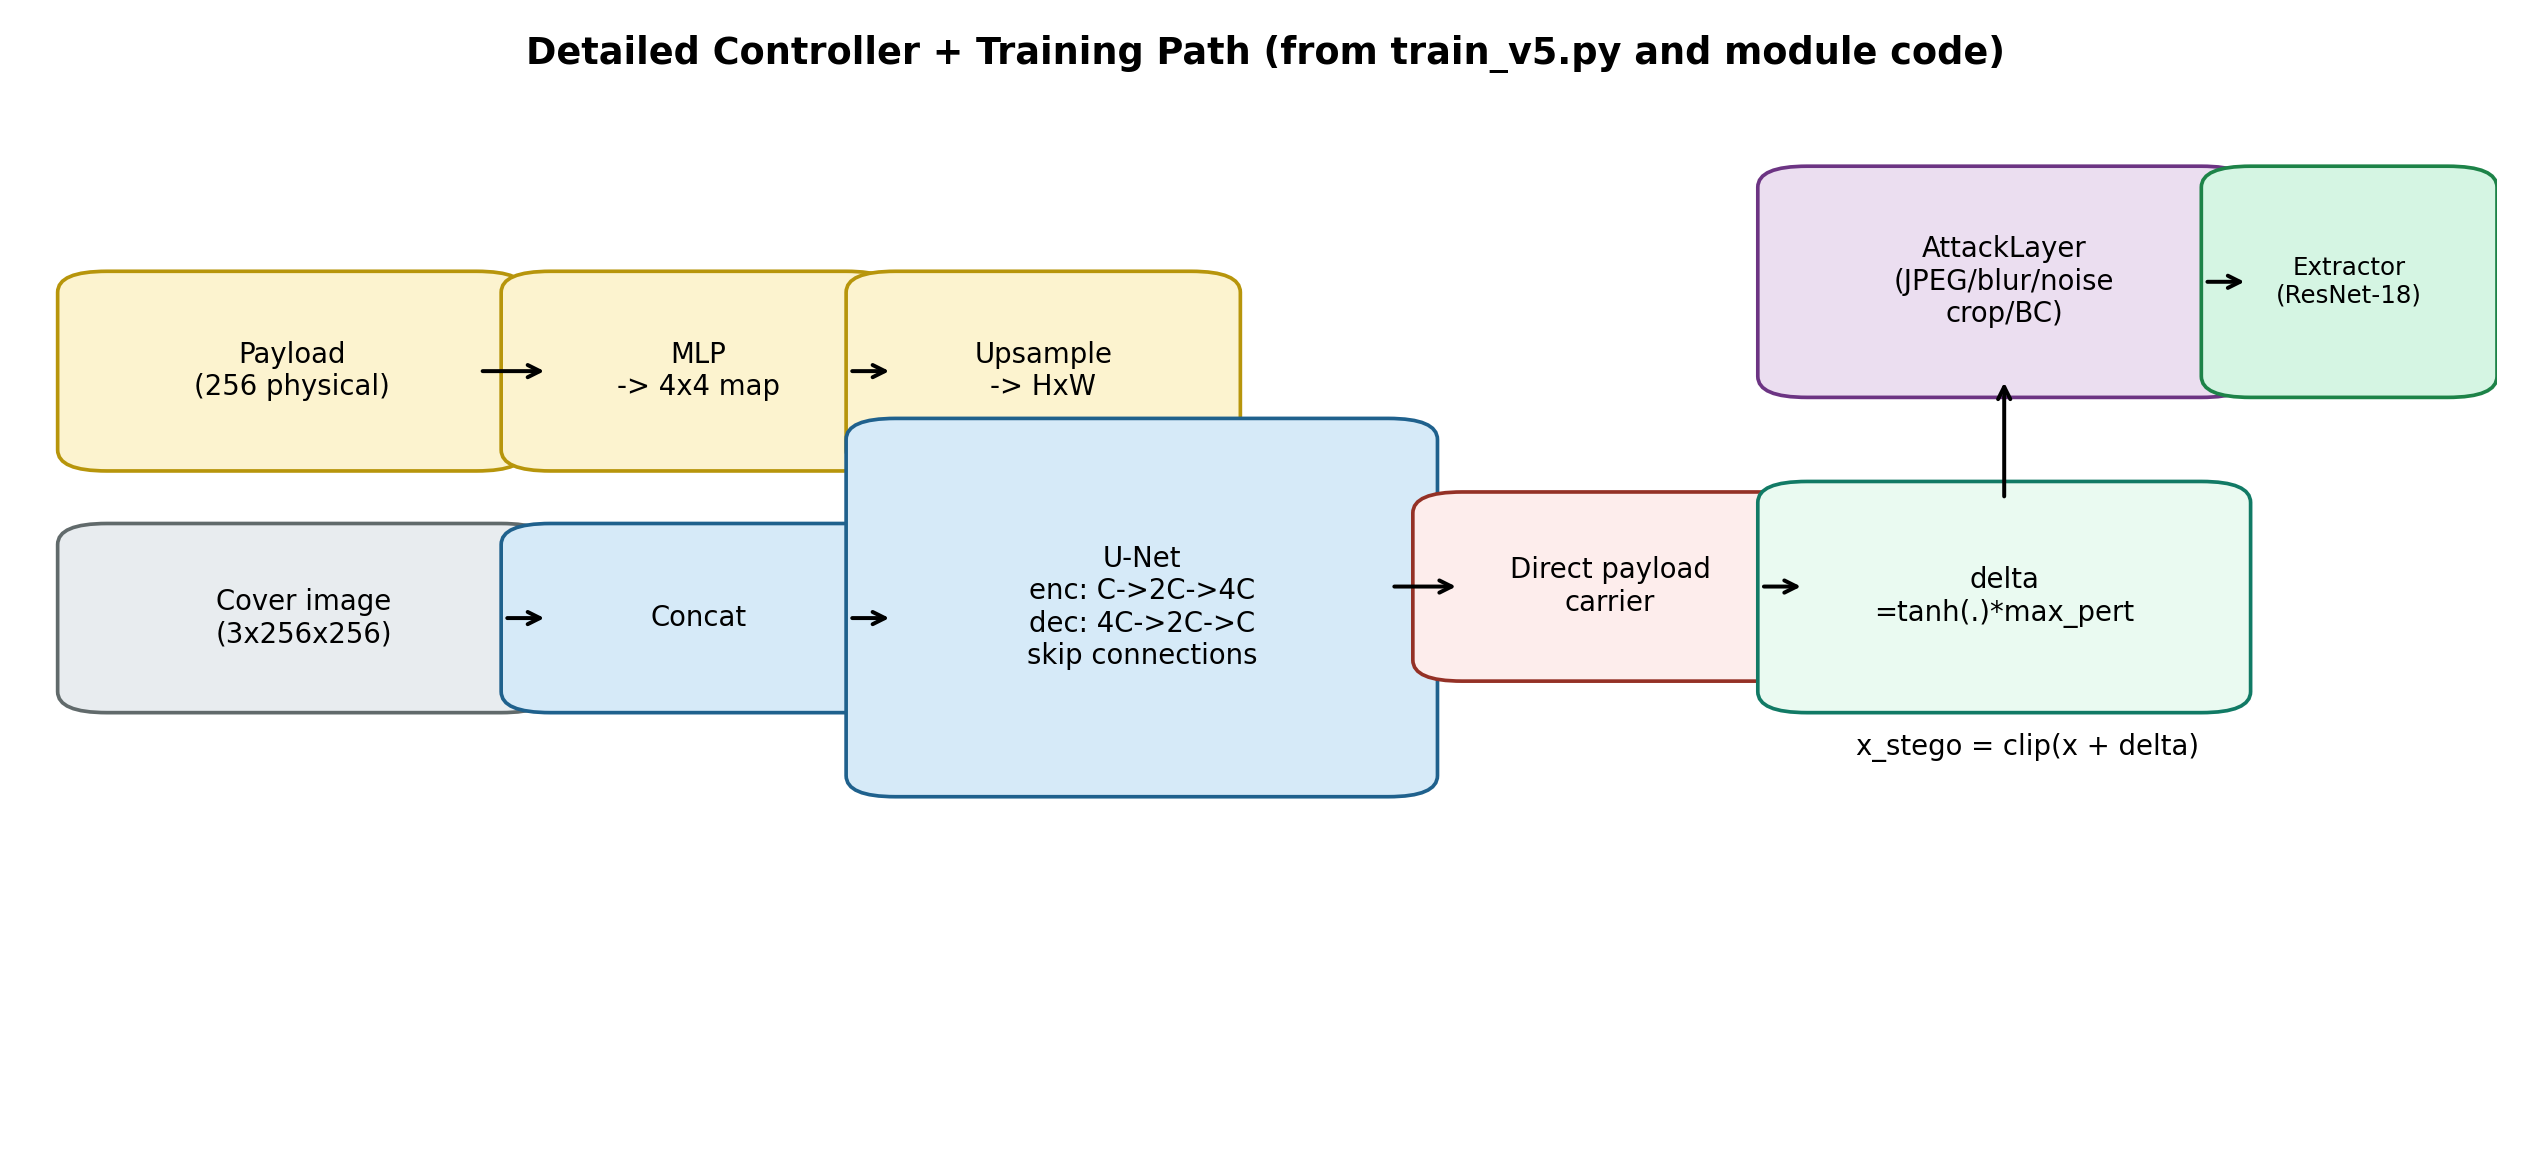
\includegraphics[width=0.95\textwidth]{figures/architecture_detail.png}
\caption{Detailed controller/extractor/training path, reflecting module-level implementation in the current repository.}
\label{fig:architecture_detail}
\end{figure*}

\subsection{Training Objectives}
From the active training scripts, the optimization combines message reconstruction and perceptual terms with optional adversarial and spectral-domain terms:
\begin{equation}
\mathcal{L} = \mathcal{L}_{\mathrm{msg}} + \lambda_{\mathrm{perc}}\mathcal{L}_{\mathrm{LPIPS}} + \lambda_{\mathrm{ctrl}}\mathcal{L}_{\mathrm{ctrl}} + \lambda_{\mathrm{adv}}\mathcal{L}_{\mathrm{adv}} + \lambda_{\mathrm{spec}}\mathcal{L}_{\mathrm{spec}} + \lambda_{\mathrm{srm}}\mathcal{L}_{\mathrm{srm}}.
\end{equation}
Not all terms are active in all lines: the autopilot v4 line and the supporting v5 line use different schedules and coefficients.

\subsection{Autopilot Search Strategy}
The TIFS autopilot rotates four variants: \emph{ber\_recovery\_clean\_first}, \emph{ber\_recovery\_curriculum}, \emph{robust\_balance}, and \emph{detectability\_harden}. Required gates are:
\begin{itemize}
\item clean BER $\leq 0.10$,
\item JPEG Q75 BER $\leq 0.20$,
\item crop Q80 BER $\leq 0.35$,
\item adaptive AUC $\leq 0.70$,
\end{itemize}
plus cross-dataset and ablation coverage checks.

\section{Experimental Protocol and Artifact Provenance}
\subsection{Primary Evidence Scope}
Primary quantitative claims are extracted from:
\begin{itemize}
\item autopilot state history and cycle outputs (cycles 1--11),
\item cycle-level evaluation JSON payloads,
\item milestone logs and run records.
\end{itemize}
The cycle-11 report uses 200 evaluation samples with cross-dataset checks on 200 CIFAR10 and 200 STL10 samples.

\subsection{Supporting Evidence Scope (v5, Explicitly Separate)}
v5 artifacts are used only for supporting analysis:
\begin{itemize}
\item short-run ablations from warm-started 8k-step variants,
\item security/statistical diagnostics from a dedicated analysis script.
\end{itemize}
These are not treated as identical to the primary v4 autopilot model.

\section{Results: Primary TIFS v4 Autopilot Line}
\subsection{Cycle Dynamics}
\begin{figure*}[t]
\centering
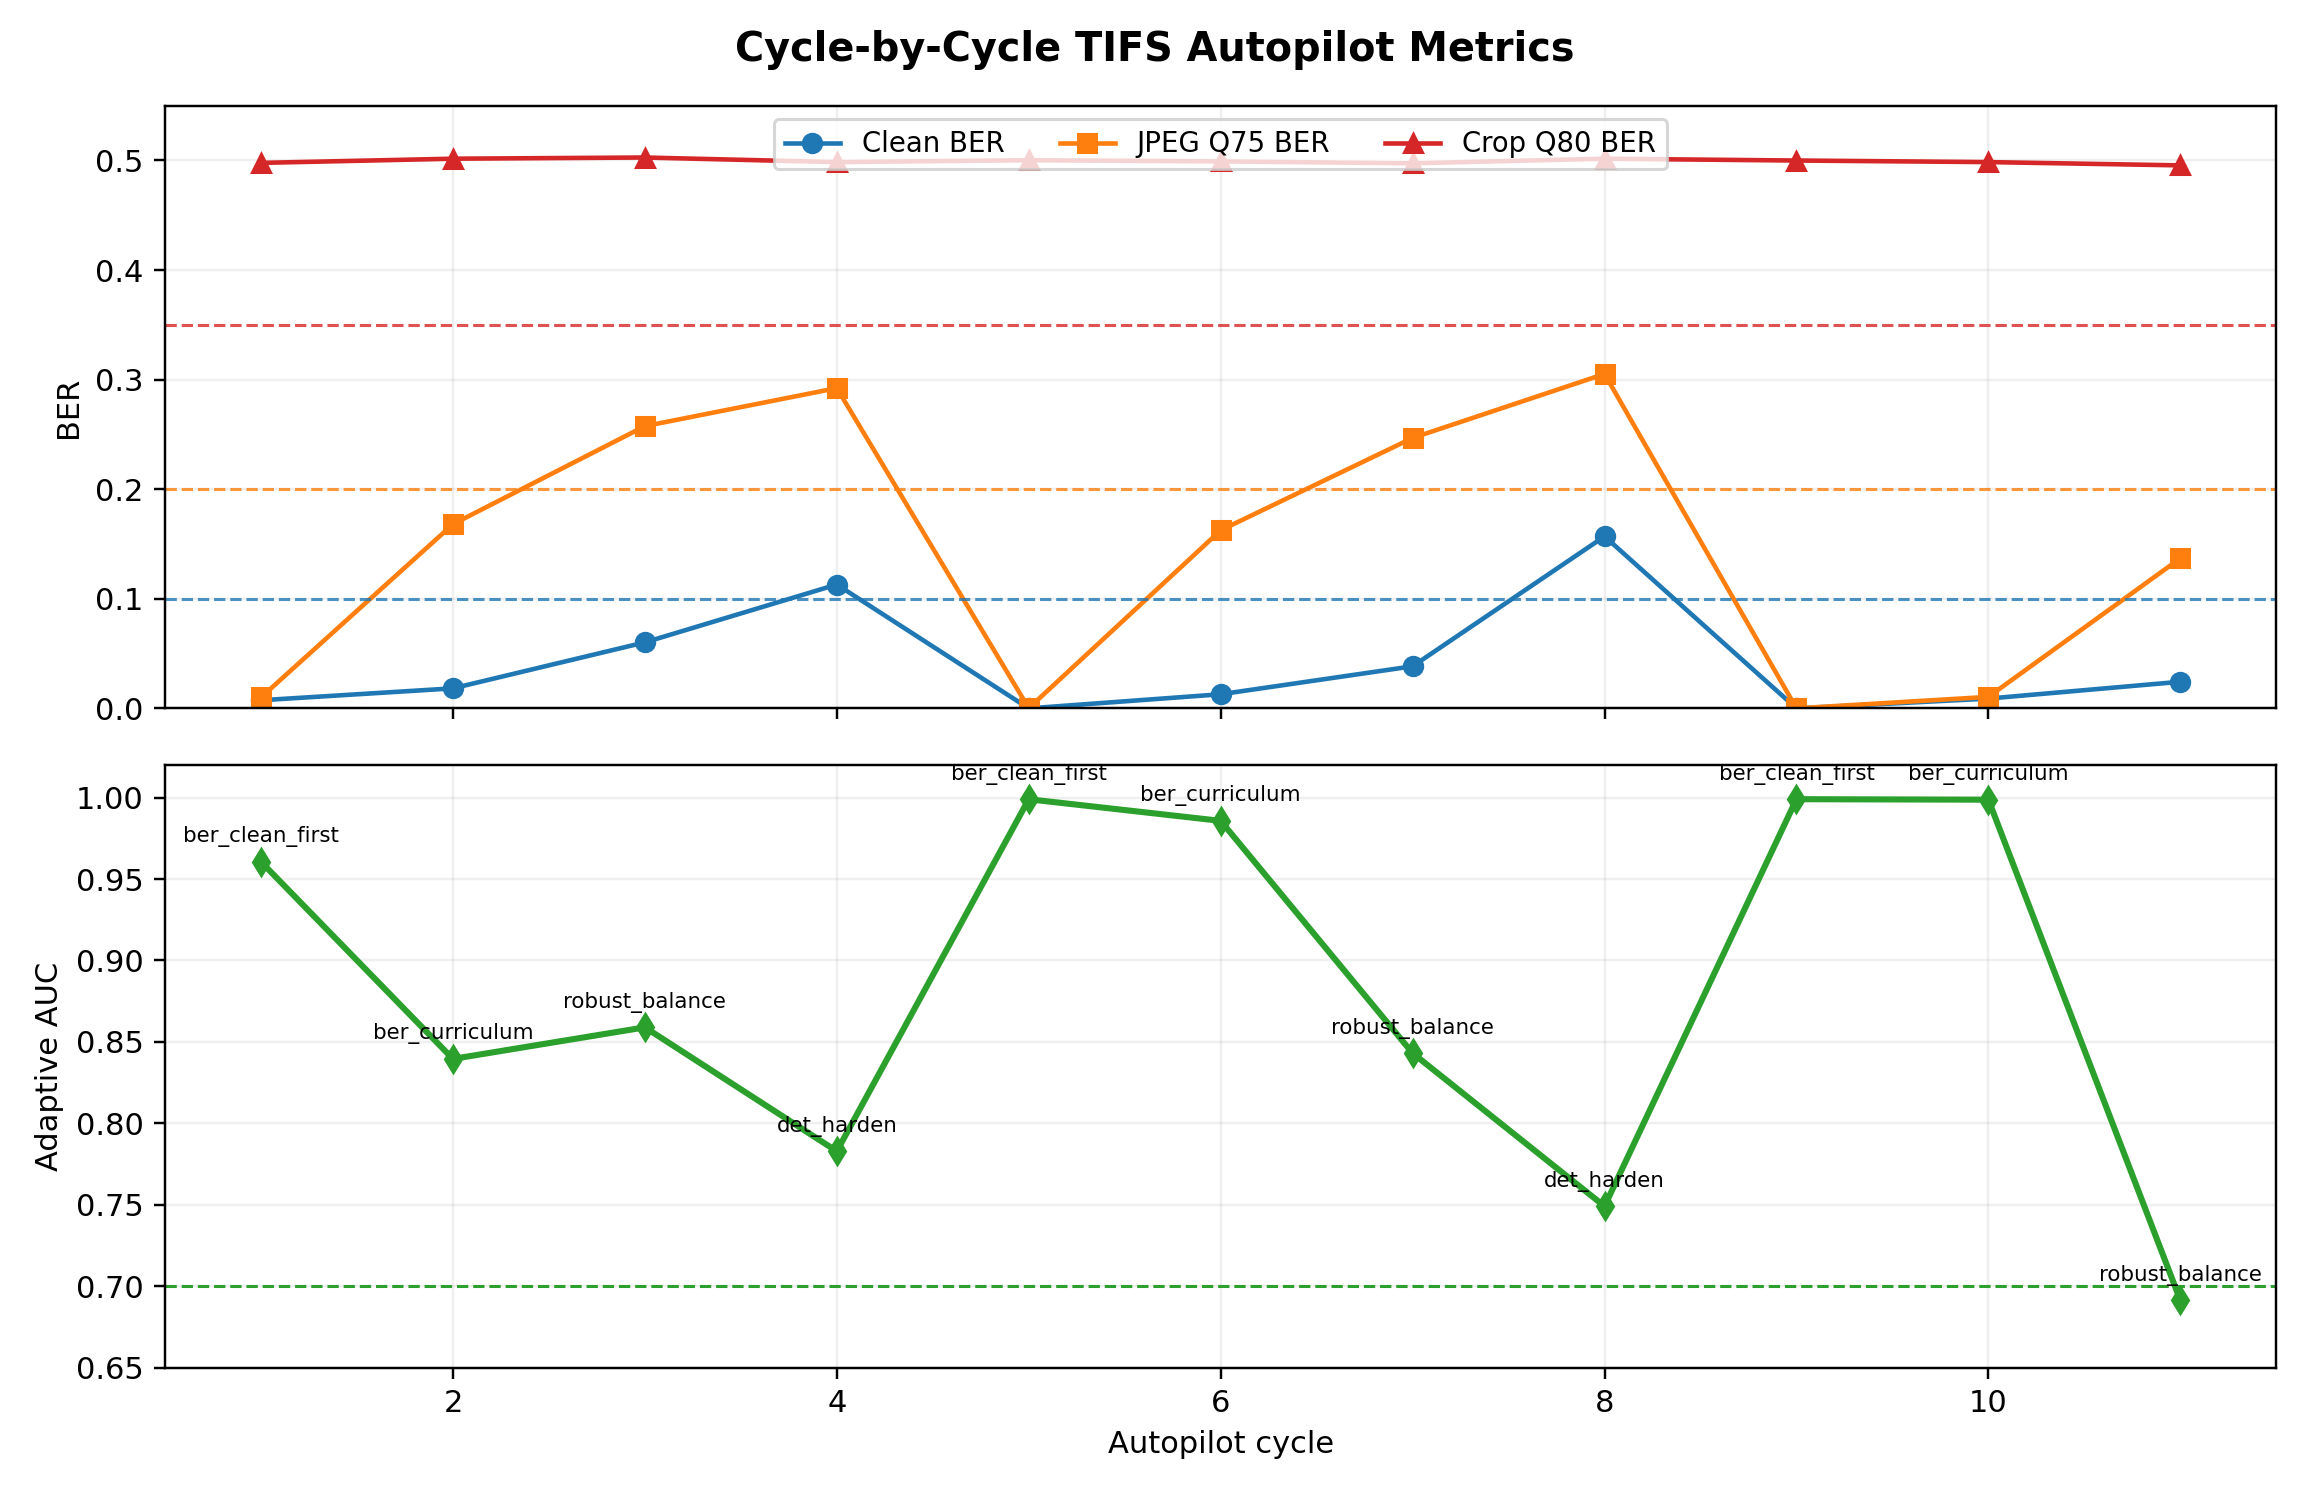
\includegraphics[width=0.95\textwidth]{figures/cycle_performance.png}
\caption{Cycle-by-cycle trajectory across clean BER, JPEG Q75 BER, crop Q80 BER, and adaptive AUC. Crop BER remains near 0.5 throughout all cycles.}
\label{fig:cycle_performance}
\end{figure*}

A key empirical pattern is a three-way tension among BER, detectability, and quality:
\begin{itemize}
\item Cycle 10 achieves very strong BER/JPEG values but remains highly detectable (AUC $\approx 0.999$).
\item Cycle 11 reduces AUC to $0.6915$ (gate pass) while BER remains acceptable and JPEG robustness is moderate.
\item Crop Q80 BER remains near random in all cycles, indicating unresolved geometric robustness.
\end{itemize}

\subsection{Main Quantitative Summary}
\begin{table}[t]
\centering
\caption{Main quantitative comparison between cycle 10 and cycle 11.}
\label{tab:main_quant}
\resizebox{\columnwidth}{!}{%
\begin{tabular}{lcccc}
\toprule
Metric & Gate & Cycle 10 & Cycle 11 & Gate@11 \\
\midrule
Clean BER & 0.100 & 0.008965 & 0.024316 & PASS \\
JPEG Q75 BER & 0.200 & 0.010527 & 0.136973 & PASS \\
Crop Q80 BER & 0.350 & 0.498457 & 0.495469 & FAIL \\
Adaptive AUC & 0.700 & 0.998700 & 0.691500 & PASS \\
PSNR (dB) & 35.000 & 32.561690 & 27.799934 & FAIL \\
\bottomrule
\end{tabular}%
}
\end{table}

Cycle 11 passes clean BER, JPEG Q75 BER, and adaptive AUC gates, but fails crop Q80 BER and PSNR target. This is the current best-balanced point in the validated run history.

\subsection{Cross-Dataset Generalization}
\begin{table}[t]
\centering
\caption{Cross-dataset evaluation from cycle 11.}
\label{tab:cross_dataset}
\resizebox{0.9\columnwidth}{!}{%
\begin{tabular}{lcc}
\toprule
Dataset & Clean BER & Crop Q80 BER \\
\midrule
CIFAR10 & 0.006309 & 0.502012 \\
STL10 & 0.123750 & 0.500664 \\
\bottomrule
\end{tabular}%
}
\end{table}

Cross-dataset clean BER is low on CIFAR10 and higher on STL10, but crop BER remains around $0.5$ on both datasets, reinforcing that the crop weakness is not dataset-specific.

\section{Ablation and Supporting Analyses}
\subsection{v5 Ablation (Supporting, Not Primary)}
\begin{figure*}[t]
\centering
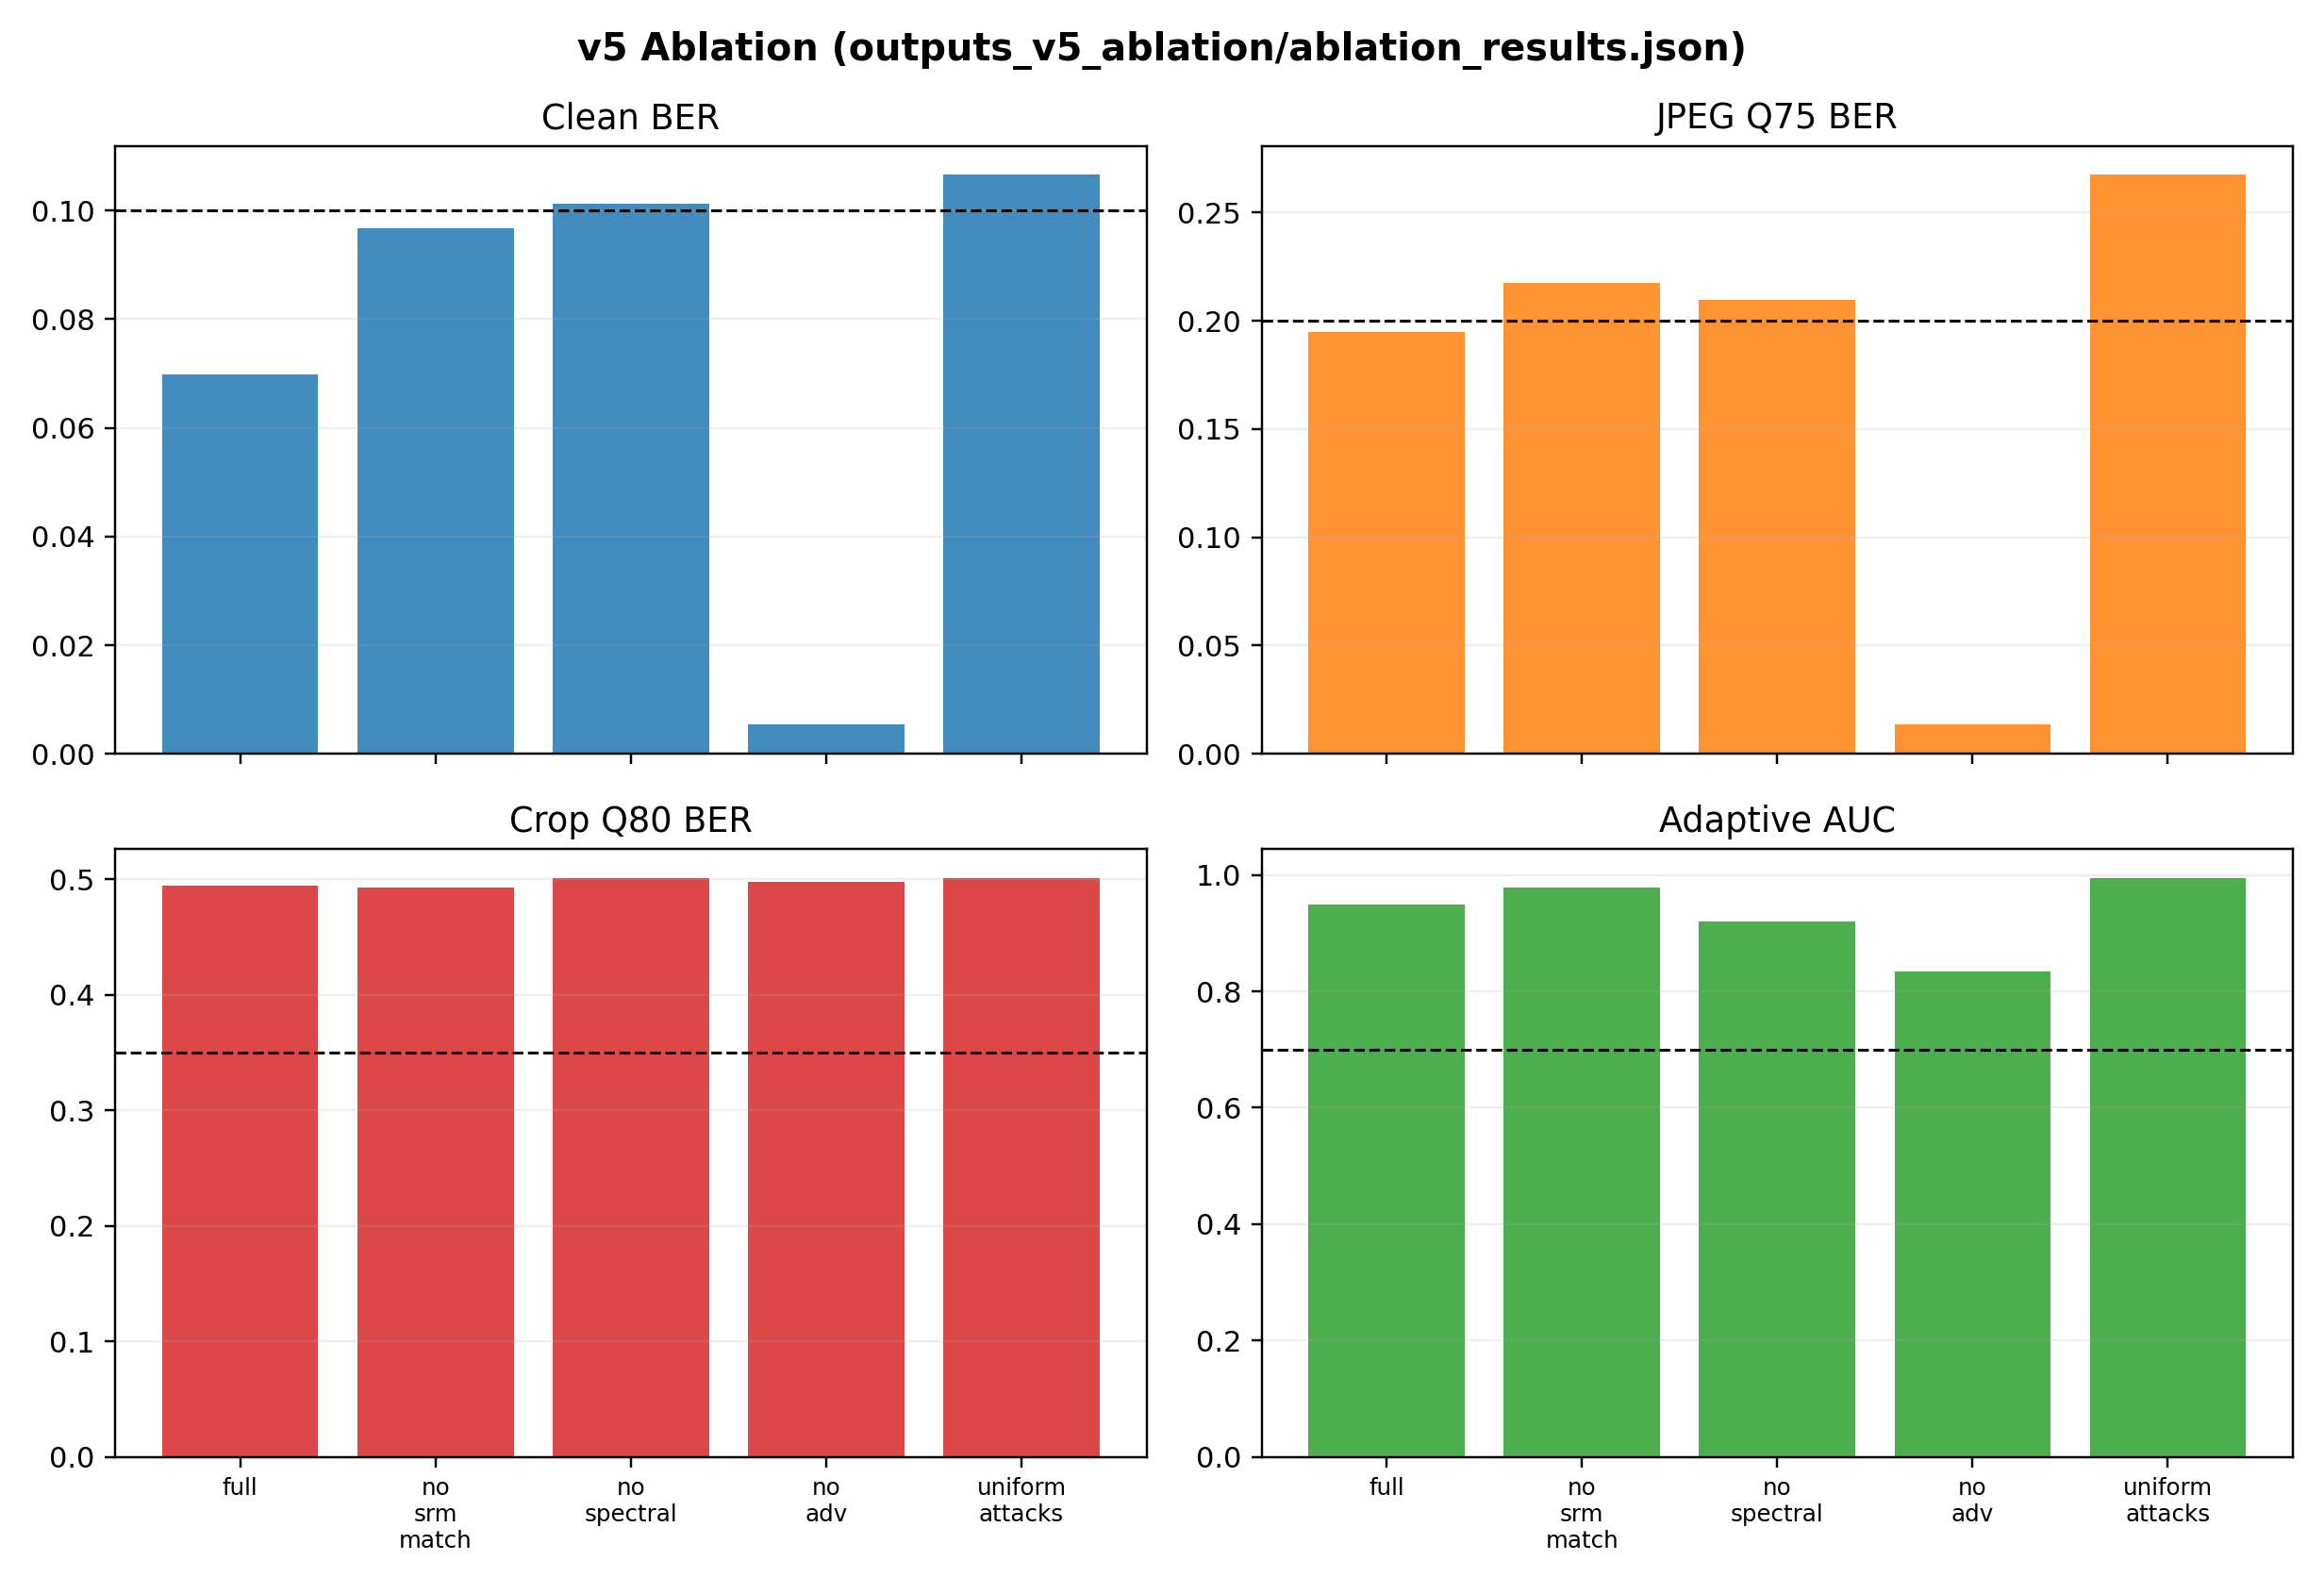
\includegraphics[width=0.95\textwidth]{figures/ablation_v5.png}
\caption{v5 short-run ablation metrics from \texttt{outputs\_v5\_ablation/ablation\_results.json}.}
\label{fig:v5_ablation}
\end{figure*}

\begin{table*}[t]
\centering
\caption{v5 ablation table (supporting evidence).}
\label{tab:v5_ablation}
\resizebox{0.75\textwidth}{!}{%
\begin{tabular}{lcccc}
\toprule
Variant & Clean BER & JPEG Q75 BER & Crop Q80 BER & AUC \\
\midrule
full & 0.069844 & 0.194922 & 0.494297 & 0.949025 \\
no\_srm\_match & 0.096797 & 0.217344 & 0.492930 & 0.977650 \\
no\_spectral & 0.101250 & 0.209727 & 0.500820 & 0.919975 \\
no\_adv & 0.005352 & 0.013672 & 0.497969 & 0.833800 \\
uniform\_attacks & 0.106563 & 0.267422 & 0.501289 & 0.995025 \\
no\_redundant & N/A & N/A & N/A & N/A \\
\bottomrule
\end{tabular}%
}
\end{table*}

Two observations are robust in the available v5 ablation logs: (i) removing adversarial training improves BER but worsens detectability, and (ii) crop BER remains near chance in all tested variants. One variant (no\_redundant) failed during run orchestration and is therefore reported as unavailable instead of imputed.

\subsection{Statistical Security Diagnostics (v5 Supporting Analysis)}
\begin{figure*}[t]
\centering
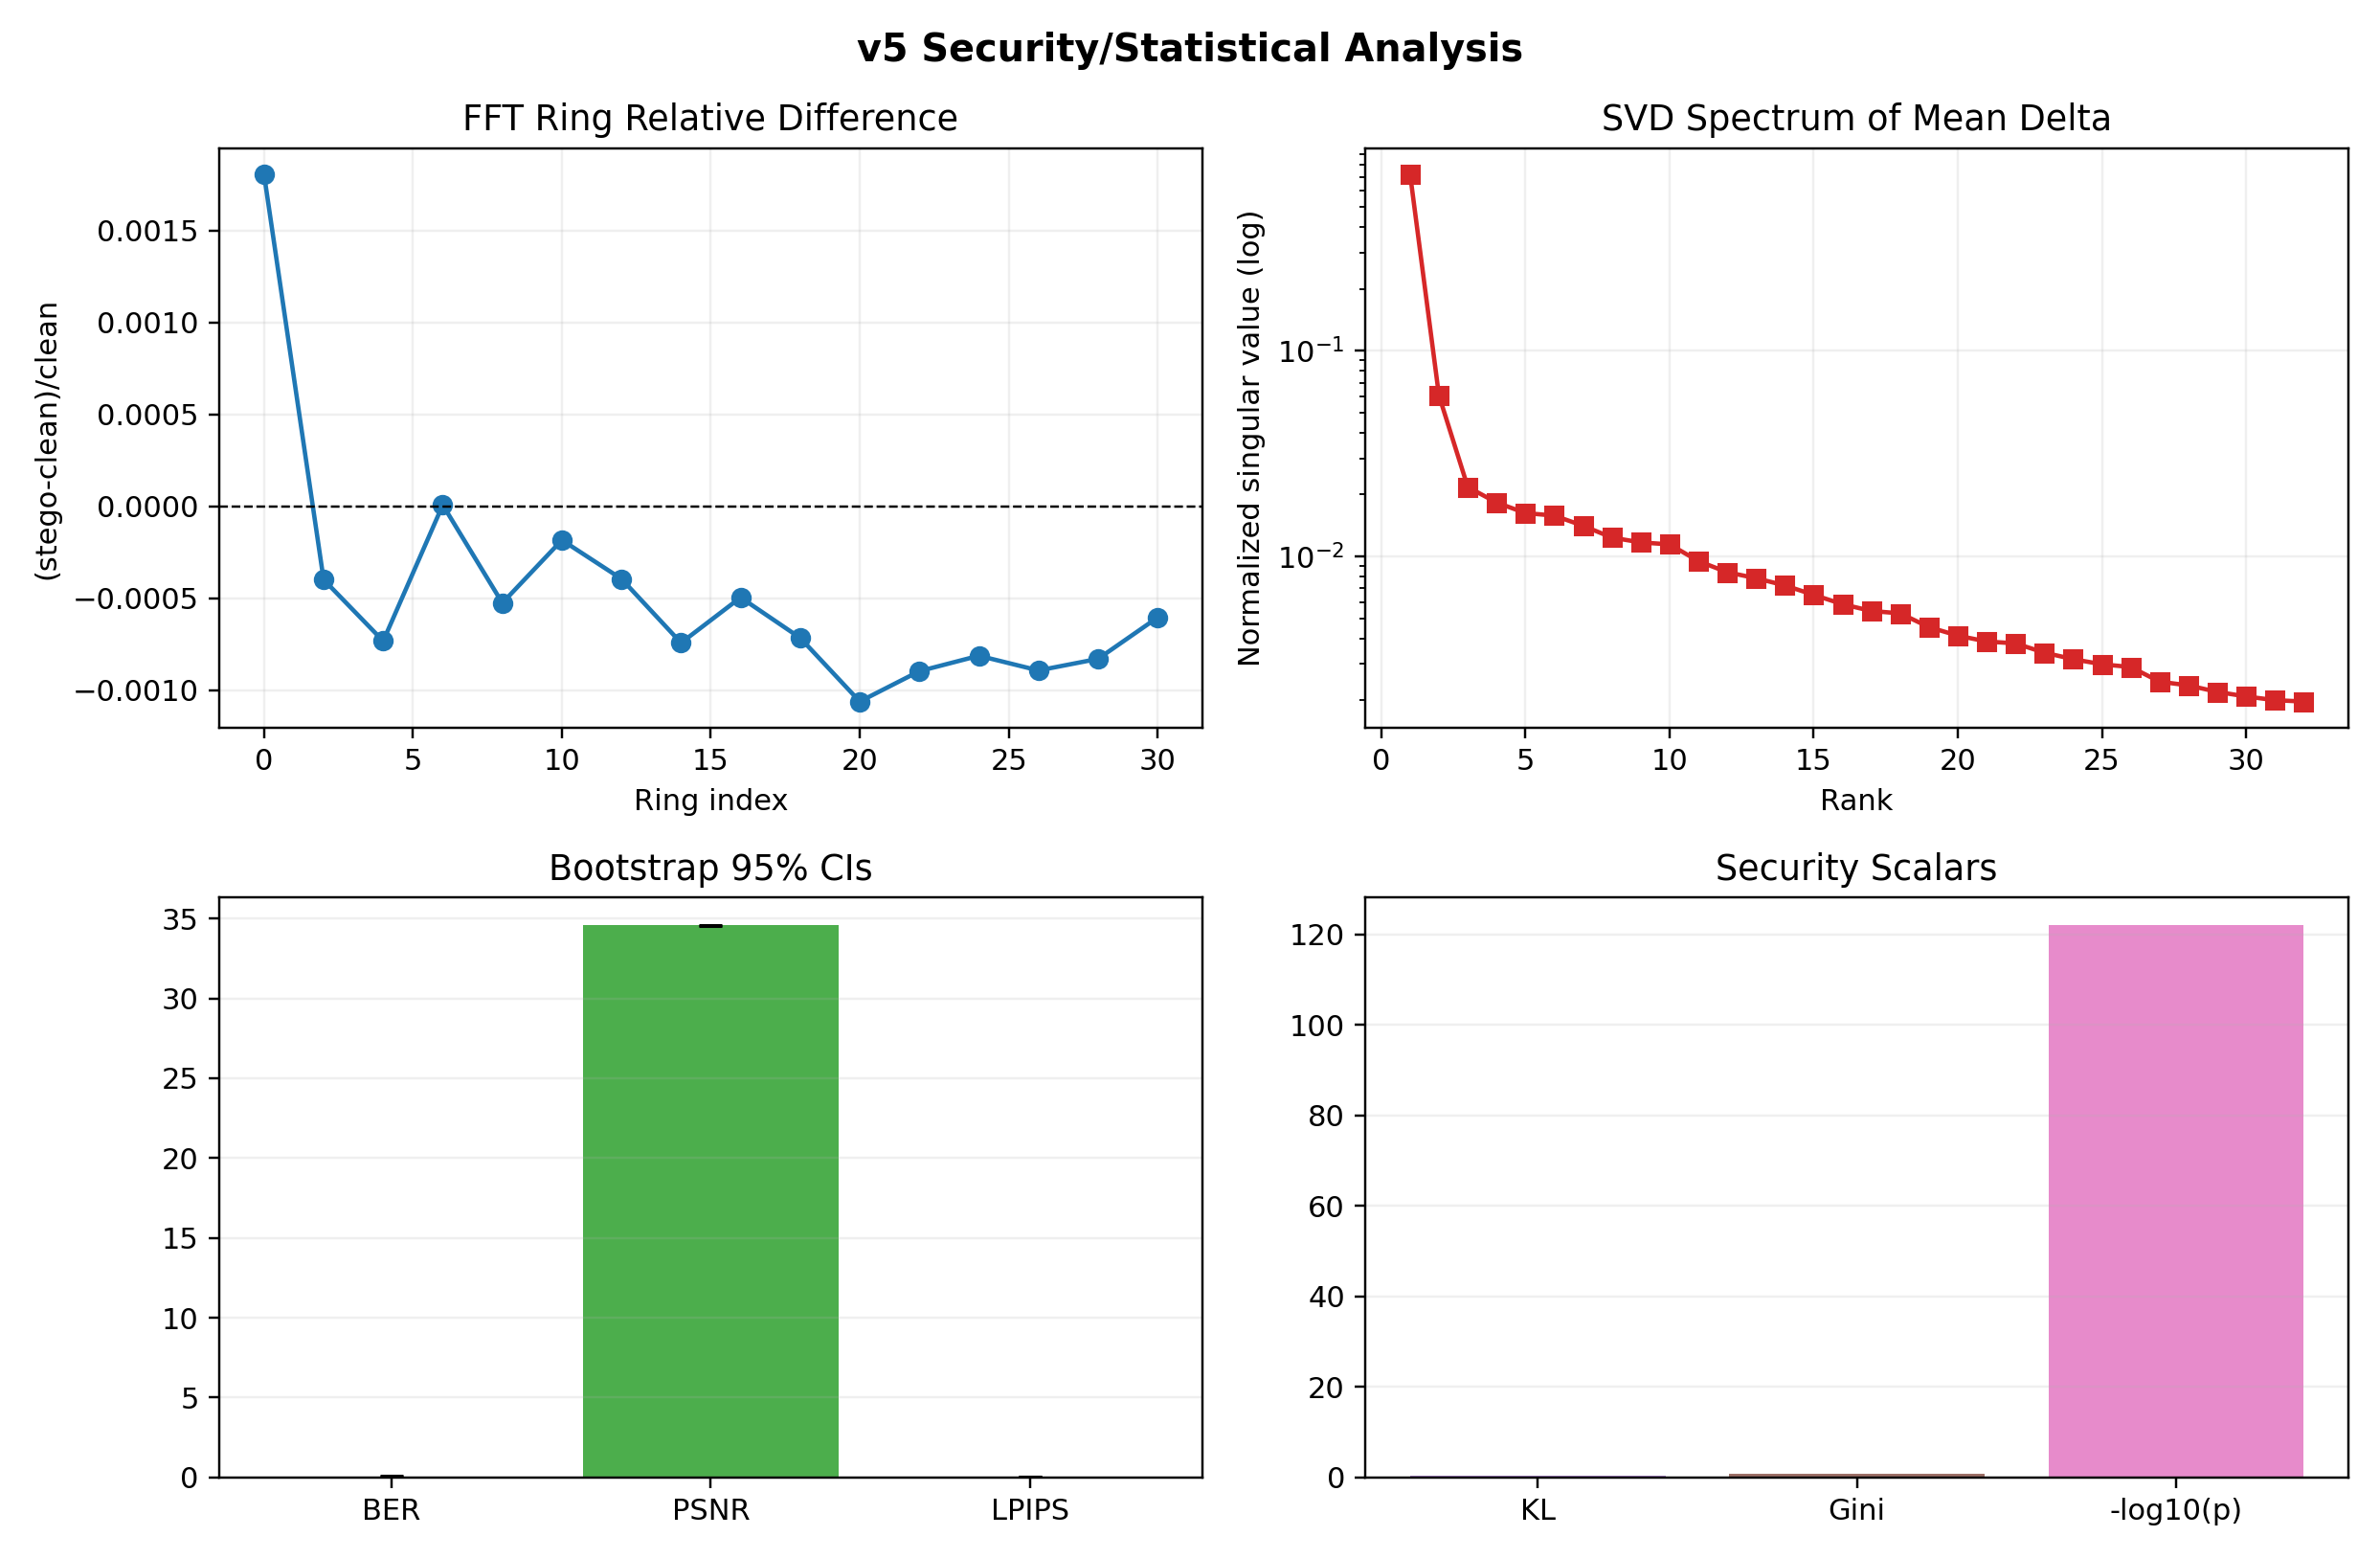
\includegraphics[width=0.95\textwidth]{figures/security_v5.png}
\caption{Security/statistical analysis from \texttt{outputs\_v5\_analysis/security\_analysis.json}.}
\label{fig:security_v5}
\end{figure*}

The v5 security report indicates mixed behavior: KL divergence between clean and stego feature fits is low ($0.417$), but spectral-histogram chi-square testing rejects the null strongly ($p\approx 1.07\times10^{-122}$), and the singular spectrum concentration is high (Gini $0.820$). Together, these results suggest residual structured artifacts despite low average perceptual shift.

\section{Failure Analysis and Limitations}
\begin{figure}[t]
\centering
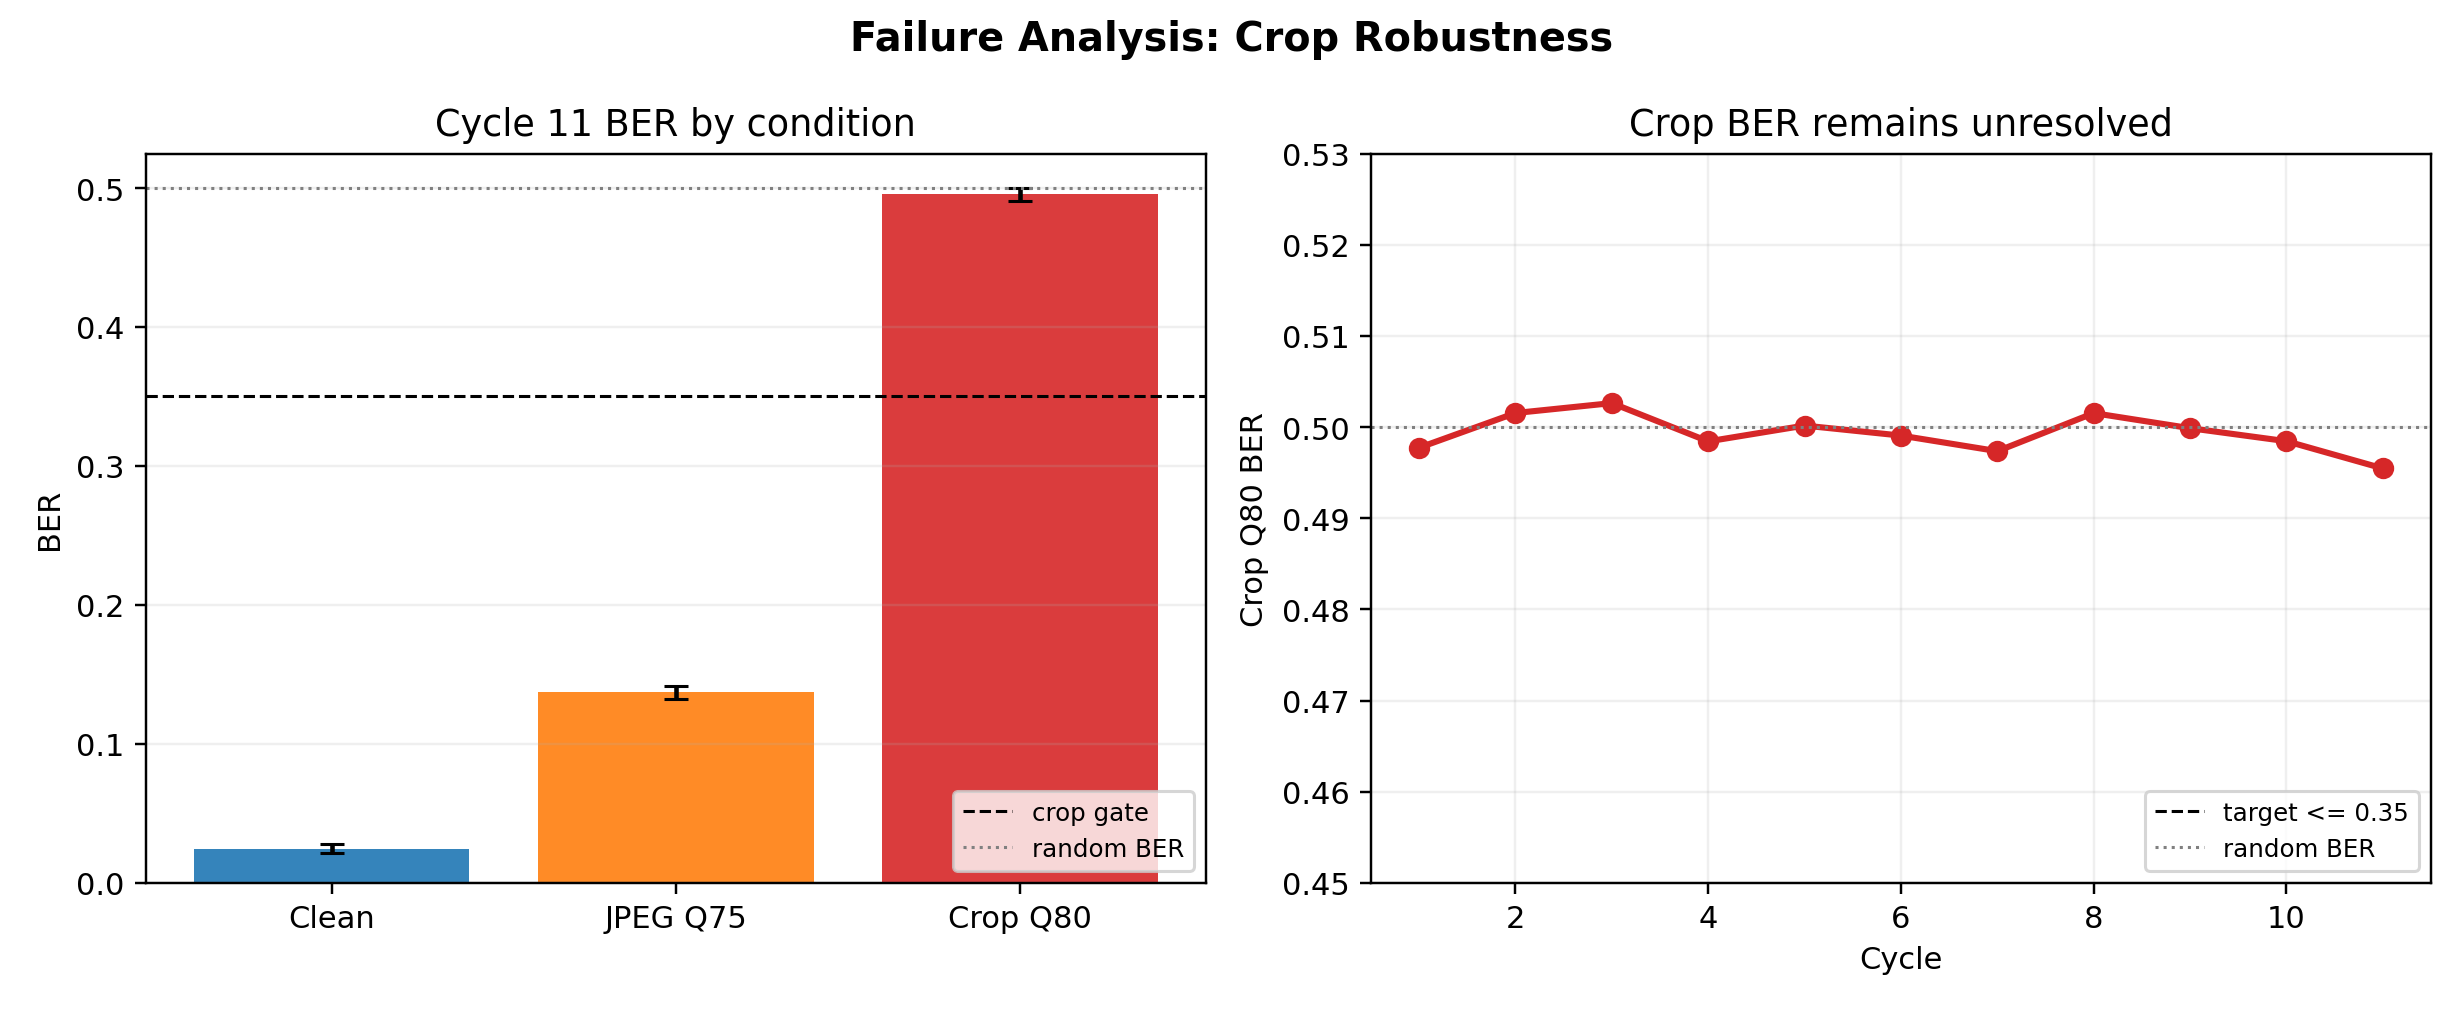
\includegraphics[width=\columnwidth]{figures/crop_failure.png}
\caption{Failure analysis centered on crop robustness. Left: cycle-11 condition-wise BER. Right: crop Q80 BER across cycles.}
\label{fig:crop_failure}
\end{figure}

\subsection{Crop Robustness Remains the Main Blocker}
Crop Q80 BER remains in the $0.495$--$0.503$ range across all cycles. This is effectively random recovery and is incompatible with deployment-oriented robustness claims.

\subsection{Quality Under Detectability-Hardened Regime}
The best detectability point (cycle 11) has PSNR $27.8$ dB, below the project quality target ($35$ dB). Current evidence does not support claiming simultaneous detectability, robustness, and quality closure.

\subsection{Residual Statistical Signature Risk}
The supporting v5 statistical tests show significant frequency-domain discrepancies and concentrated perturbation modes. This aligns with the crop failure and indicates additional regularization and/or encoding redesign are needed.

\subsection{Current Scope Boundaries}
The present manuscript is evidence-faithful to local artifacts and does not claim external benchmark superiority or state of the art. Several bibliographic entries (especially recent diffusion steganography papers) should be metadata-verified before final camera-ready submission.

\section{Conclusion}
Using current repository artifacts as source of truth, DSCSP now demonstrates one meaningful milestone: adaptive steganalysis AUC can reach the target regime (cycle 11: $0.6915$) while maintaining non-trivial BER performance (clean BER $0.0243$, JPEG Q75 BER $0.1370$). At the same time, the central blocker is unresolved: crop Q80 BER remains near random, and quality at the best detectability point is below target.

The practical outcome is clear. The project has moved from optimistic draft claims to a measurable, reproducible frontier with explicit pass/fail boundaries. This is a stronger foundation for future TIFS-ready iterations than metric inflation or model-line conflation. The immediate next research direction is crop-first architecture and training redesign with detectability retained as a hard constraint.

\bibliographystyle{IEEEtran}
\begin{thebibliography}{99}

\bibitem{bengio2013estimating}
Y.~Bengio, N.~L{\'e}onard, and A.~Courville, ``Estimating or propagating gradients through stochastic neurons for conditional computation,'' \emph{arXiv preprint arXiv:1308.3432}, 2013.

\bibitem{boroumand2019deep}
M.~Boroumand, M.~Chen, and J.~Fridrich, ``Deep residual network for steganalysis of digital images,'' \emph{IEEE Trans. Inf. Forensics Security}, vol.~14, no.~5, pp.~1181--1193, 2019.

\bibitem{cox2007digital}
I.~Cox, M.~Miller, J.~Bloom, J.~Fridrich, and T.~Kalker, \emph{Digital Watermarking and Steganography}, 2nd~ed. Morgan Kaufmann, 2007.

\bibitem{fridrich2012rich}
J.~Fridrich and J.~Kodovsk{\'y}, ``Rich models for steganalysis of digital images,'' \emph{IEEE Trans. Inf. Forensics Security}, vol.~7, no.~3, pp.~868--882, 2012.

\bibitem{goodfellow2014generative}
I.~Goodfellow \emph{et al.}, ``Generative adversarial nets,'' in \emph{Proc. NeurIPS}, 2014, pp.~2672--2680.

\bibitem{he2016deep}
K.~He, X.~Zhang, S.~Ren, and J.~Sun, ``Deep residual learning for image recognition,'' in \emph{Proc. IEEE CVPR}, 2016, pp.~770--778.

\bibitem{ho2020denoising}
J.~Ho, A.~Jain, and P.~Abbeel, ``Denoising diffusion probabilistic models,'' in \emph{Proc. NeurIPS}, 2020, pp.~6840--6851.

\bibitem{holub2012designing}
V.~Holub and J.~Fridrich, ``Designing steganographic distortion using directional filters,'' in \emph{Proc. IEEE WIFS}, 2012, pp.~234--239.

\bibitem{holub2014universal}
V.~Holub, J.~Fridrich, and T.~Denemark, ``Universal distortion function for steganography in an arbitrary domain,'' \emph{EURASIP J. Inf. Security}, vol.~2014, no.~1, pp.~1--13, 2014.

\bibitem{miyato2018spectral}
T.~Miyato, T.~Kataoka, M.~Koyama, and Y.~Yoshida, ``Spectral normalization for generative adversarial networks,'' in \emph{Proc. ICLR}, 2018.

\bibitem{peng2023stegodiffusion}
W.~Peng, Z.~Li, Y.~Chen, and Z.~Wang, ``Generative steganography diffusion,'' \emph{arXiv preprint arXiv:2305.03472}, 2023.

\bibitem{pevny2010using}
T.~Pevn{\'y}, T.~Filler, and P.~Bas, ``Using high-dimensional image models to perform highly undetectable steganography,'' in \emph{Information Hiding}. Springer, 2010, pp.~161--177.

\bibitem{shin2017jpeg}
R.~Shin and D.~Song, ``JPEG-resistant adversarial images,'' in \emph{NeurIPS Workshop on Machine Learning and Computer Security}, 2017.

\bibitem{song2020denoising}
J.~Song, C.~Meng, and S.~Ermon, ``Denoising diffusion implicit models,'' in \emph{Proc. ICLR}, 2021.

\bibitem{wei2023diffusionstego}
R.~Wei, C.~Wen, Y.~Xue, and T.~Wang, ``Diffusion-Stego: Training-free diffusion generative steganography via message projection,'' \emph{arXiv preprint arXiv:2305.18726}, 2023.

\bibitem{zhang2018unreasonable}
R.~Zhang, P.~Isola, A.~A.~Efros, E.~Shechtman, and O.~Wang, ``The unreasonable effectiveness of deep features as a perceptual metric,'' in \emph{Proc. IEEE CVPR}, 2018, pp.~586--595.

\bibitem{zhang2019steganogan}
K.~A.~Zhang, A.~Cuesta-Infante, L.~Xu, and K.~Veeramachaneni, ``SteganoGAN: High capacity image steganography with GANs,'' \emph{arXiv preprint arXiv:1901.03892}, 2019.

\bibitem{zhang2024ldstega}
J.~Zhang, Y.~Qin, Z.~Liu, and T.~Wang, ``LDStega: Practical and robust generative image steganography based on latent diffusion models,'' in \emph{Proc. ACM Multimedia}, 2024.

\bibitem{zhao2024dero}
J.~Zhao, Y.~Liu, and X.~Zhang, ``DERO: Diffusion-model-erasure robust watermarking,'' in \emph{Proc. ACM Multimedia}, 2024.

\bibitem{zhu2018hidden}
J.~Zhu, R.~Kaplan, J.~Johnson, and L.~Fei-Fei, ``HiDDeN: Hiding data with deep networks,'' in \emph{Proc. ECCV}, 2018, pp.~657--672.

\end{thebibliography}

\end{document}
